\documentclass{article}
\usepackage[french]{babel}
\usepackage[utf8]{inputenc}
\usepackage{graphicx}
\usepackage{dejavu}
\renewcommand*\familydefault{\sfdefault} %% Only if the base font of the document is to be sans serif
\usepackage[T1]{fontenc}

\usepackage{geometry}
\geometry{a4paper,headheight=16pt,tmargin=25mm,
          bmargin=25mm,lmargin=20mm,rmargin=20mm}

\usepackage{fancyhdr}
\usepackage{lastpage}

\usepackage{hyperref}
 
\pagestyle{fancy}
\fancyhf{}
\lhead{\footnotesize Première STI2D\\Tronc commun}
\chead{\large AP Numérisation de l'information : codage binaire}
\lfoot{Lycée Blaise Pascal}
\rfoot{\thepage/\pageref{LastPage}}

\renewcommand{\headrulewidth}{1pt}
\renewcommand{\footrulewidth}{1pt}

\begin{document}
\begin{center}
%	\begin{minipage}[b]{.6\linewidth}
%	\end{minipage}
%	\hfill
%	\begin{minipage}[b]{.3\linewidth}
%		\scriptsize
%		\begin{Form}
%			\TextField[name=nom,width=10em,]{Nom:}\\
%			\TextField[name=prenom,width=10em]{Prénom:}\\
%			\TextField[name=classe,width=10em]{Classe:}\\
%		\end{Form}
%	\end{minipage}
	\begin{flushright}
		\begin{Form}
			\TextField[name=nom,width=10em,default=Nom]{Nom:}\\
			\TextField[name=prenom,width=10em,default=Prénom]{Prénom:}\\
			\TextField[name=classe,width=10em,default=Classe]{Classe:}\\
		\end{Form}
	\end{flushright}

	\vspace{1em}
	\Large
	\textbf{Objectif:} Comment l'ordinateur fait-il pour coder une image?

	\vspace{2em}
	\large
	\textbf{Consigne}: Vous formaliserez vos réponses dans ce document numérique

	\vspace{2em}
	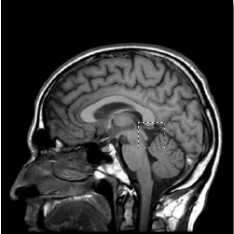
\includegraphics[width=.3\linewidth]{./figures/irm1.png}
	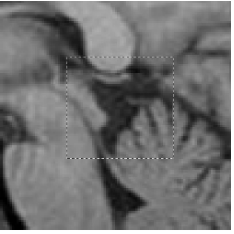
\includegraphics[width=.3\linewidth]{./figures/irm2.png}
	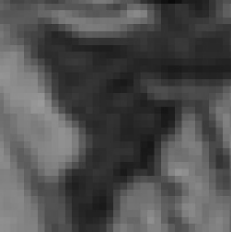
\includegraphics[width=.3\linewidth]{./figures/irm3.png}
\end{center}

\section{Codage d'une image numérique matricielle}
\paragraph{Q1:}
À partir de l'article \href{https://fr.wikipedia.org/wiki/Pixel}{wikipédia sur le pixel}, indiquer:
\begin{itemize}
	\item sa définition;
	\item son abréviation;
	\item la locution anglaise d’où provient le nom \og{}pixel\fg{} ainsi que sa traduction française.
\end{itemize}

\vspace{1em}
\begin{Form}
	\TextField[name=r1,width=\linewidth,height=5em,multiline=true]{}
\end{Form}

\paragraph{Q2:}
Ouvrir le fichier image \og{}stop P5.PGM\fg{} à l'aide du logiciel de visualisation de fichier graphique XNVIEW. 
En zoomant au maximum, indiquer pour l'image considérée:
\begin{itemize}
	\item la largeur (en px);
	\item la hauteur (en px);
	\item le nombre total de pixels.
\end{itemize}

\vspace{1em}
\begin{Form}
	\TextField[name=r1,width=\linewidth,height=5em,multiline=true]{}
\end{Form}

\begin{minipage}[b]{.08\linewidth}
	
\includegraphics[width=\linewidth]{./figures/info.png}
\end{minipage}
\hfill
\begin{minipage}[b]{.85\linewidth}
	Pour observer le codage du fichier tel qu’il est dans l’ordinateur, il faut ouvrir l’image avec	un éditeur hexadécimal.
	\vspace{.7em}
\end{minipage}
Tout en laissant ouverte l'image dans Xnview, ouvrir le fichier \og{}stop P5.PGM\fg{}
à l'aide de l’éditeur hexadécimal \og{}Free Hex Editor Neo\fg{} en juxtaposant sur l'écran du PC les 2 représentations (voir ci-dessous).

\newpage
prout
\end{document}
